% accentcolor - https://www.tu-darmstadt.de/media/medien_stabsstelle_km/services/medien_cd/das_bild_der_tu_darmstadt.pdf (pages 17-18)
% amsmath	- formatting math stuff	(ftp://ftp.ams.org/pub/tex/doc/amsmath/amsldoc.pdf)
% enumitem	- formatting enumerates	(http://ftp.uni-erlangen.de/ctan/macros/latex/contrib/enumitem/enumitem.pdf)
% graphicx	- images				(http://ctan.space-pro.be/tex-archive/macros/latex/required/graphics/grfguide.pdf)
% lipsum	- lorem ipsum			(ftp://ftp.fu-berlin.de/tex/CTAN/macros/latex/contrib/lipsum/lipsum.pdf)
% listings	- source code			(http://texdoc.net/texmf-dist/doc/latex/listings/listings.pdf)
% mathtools	- amsmath extension		(ftp://ftp.fu-berlin.de/tex/CTAN/macros/latex/contrib/mathtools/mathtools.pdf)
% parskip	- splittitle 
\documentclass[11pt, accentcolor=tud1c]{tudreport}	
\usepackage[english]{babel}
\usepackage[utf8]{inputenc}
\usepackage{amsmath, enumitem, graphicx, hyperref, lipsum, listings, mathtools, parcolumns, pdfpages}

% https://scm.informatik.tu-darmstadt.de/news/129-technical-documentation-sample


% Specifying new commands
\newcommand{\titlerow}[2]{
    \begin{parcolumns}[colwidths={1=.15\linewidth}]{2}
        \colchunk[1]{#1:}
        \colchunk[2]{#2}
    \end{parcolumns}
    \vspace{0.2cm}
}

% configuring title
\title{Internet-Praktikum: Telekooperation}
\setinstitutionlogo{./res/logo.pdf}

\subtitle{
	\titlerow{Project}{Sechzehn}
	\titlerow{Team Bravo}{Alexander Geiß {\normalsize(alexanderhelmut.geiss@stud.tu-darmstadt.de)}, \\ 
	                      Lukas Klein {\normalsize(lukas.klein@stud.tu-darmstadt.de)},  \\ 
	                      Martin Lichtblau {\normalsize(martin.lichtblau@stud.tu-darmstadt.de)}, \\ 
	                      Johannes Semsch {\normalsize(johannesmaximilianchristian.semsch@stud.tu-darmstadt.de)}, \\ 
	                      Tim Walter {\normalsize(tim.walter.10@stud.tu-darmstadt.de)}}
}



% document 
\begin{document}

\maketitle
\tableofcontents

\chapter{Motivation}\label{ch:motivation}
% ! max. 1 page !


\chapter{Overview}\label{ch:overview}
% ! image demanded !
In this section we present the architecture we used and thereby how our components interact with each other. We then briefly describe which technologies we chose, and why we chose them.
\section{Architecture}\label{sec:architecture}
% components and their interaction
\subsection{Interaction of Components}
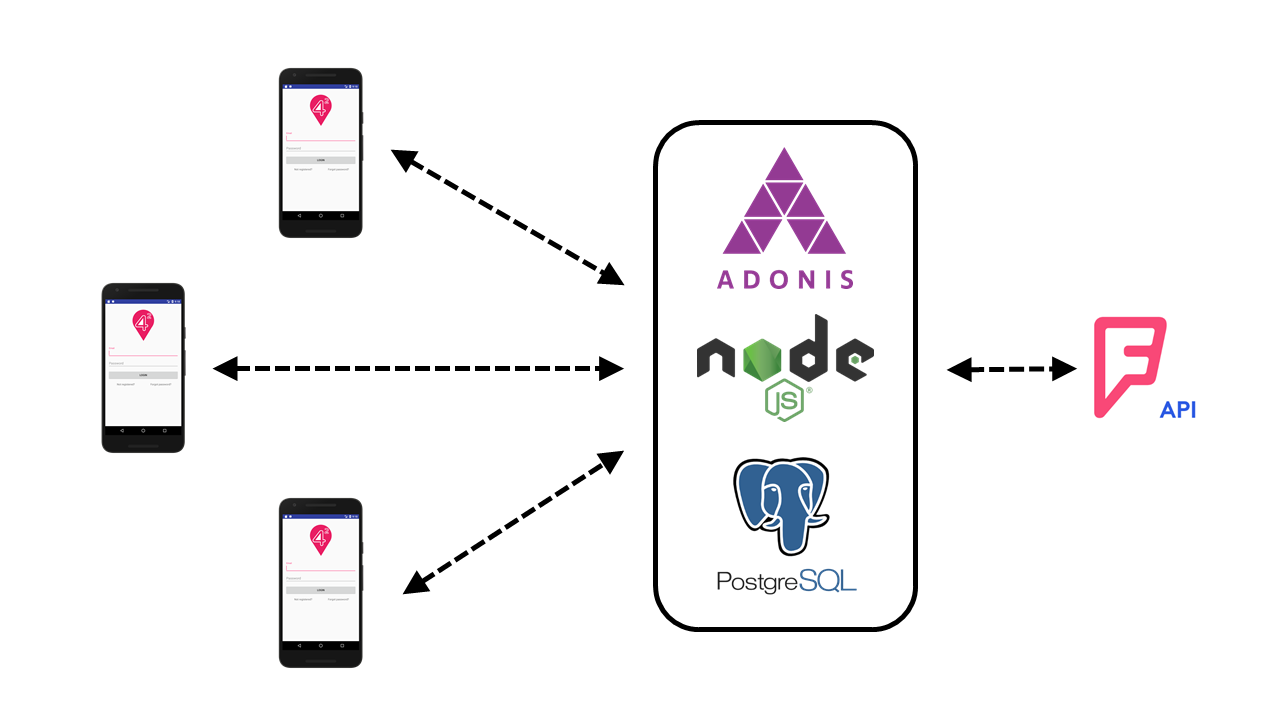
\includegraphics[scale=0.5]{./res/architecture.png}
\subsection{ERM}
\subsection{UML Diagram}
\section{Server}\label{sec:server}
To host our server we use the Heroku Cloud Application Platform\cite{heroku}. Heroku provides us a PostgreSQL\cite{postgresql} database service and an nodejs execution environment. Furthermore it offers access to Cloudinary\cite{cloudinary} image backend. The Cloudinary service can be used as plugin within heroku.
\subsection{Node.js}
\cite{nodejs}
\subsection{AdonisJs}\label{sec:adonisjs}
\cite{adonisjs}
\subsection{PostgreSQL}
PostgreSQL\cite{postgresql} is an open-source relational database management system. It is possible to add new data types and functions in PostgreSQL. Amongst other things we implemented a function to compute the Great-circle distance\cite{greatcircledist}. The Great-circle distance is necessary to compute distances on spheres and therefore to compute distances on the earth. Moreover native programming interfaces exist for many languages. Since Heroku also has a PostgreSQL plugin, that was our way to go.
\subsection{JSON Web Tokens}\label{sec:json_web_tokens}
The Authentication in our project is done with JSON Web Tokens(JWTs)\cite{jwt}.

\section{Client}\label{sec:client}
\subsection{Android Data Binding}
\cite{databinding}
\subsection{Retrofit}
\cite{retrofit}
\subsection{GSON}
\cite{gson}
\subsection{ChatKit}
\cite{chatkit}

% TODO
% technologies used
% interfaces
% pls explain your design decisions!
% pls explain the particular components, interfaces,..(e.g., app, database, API,..) in detail.


\chapter{App and Feature Explanation}\label{ch:app_and_feature_explanation}

\section{System Requirements}\label{sec:system_requirements}
%minSDK 23 %% compileSDK 25 ??? %% Permissions and justification why they are necessary
To run the app with all features Android Marshmallow (APK 23) is needed. 
In this section we briefly describe which permissions are requested by the app and why they are necessary.
\begin{enumerate}
\item permission to take pictures and videos: This permission allows us to take pictures and add them to venues.
\item permission to get access to pictures, media, and files on the device: Normally users use profile pictures for more than one app, what makes it necessary to load those pictures from the gallery. This permission is further needed to store the users login credentials on the phone.
\item permission to have access to the location of the device: The whole concept of the app is based on the users location. The location is necessary to see users and venues in the surroundings. With an incognito switch however, the user can hide his account from the map.
\end{enumerate}

\section{Get Started}
%%%download and install the APK%%%
To install the app you have to download it from the app from our web page \cite{app}. After you downloaded it you have to install it. If your phone has not the permission to install apps from third parties, you have to allow your phone to install apps from third parties. This is described by the following steps (some phones will directly lead you to step 3):
\begin{enumerate}
\item go to Settings
\item choose Security
\item scroll to Unknown sources
\item allow the installation from unknown sources
\end{enumerate} 
If your phone is allowed to install apps from third parties, the phone asks you to install the app. To do so tap on install. Now you have installed the app successfully. Have fun and enjoy the usage.

\section{Features}
We only list the bonus features because the mandatory features have to be fullfilled.
\begin{enumerate}
\item account verification with an email: \\
After registering the email has to be verified first. Without this verification, the user cannot use the app.
\item open the links from the emails: \\
After resetting your password or registering a new account the user receives an email containing a link. Our app is able to handle this link on click. This means that no verification code must be entered and no external browser is necessary to do this.
\item Resource-efficient location updating: \\
To treat the users battery with care, we use the Google Location Services. If another app on the system requests the location via those location services, we use the new location if it is more accurate. If there hasn't been a request for more than two minutes our app self starts a request to the location services. More inaccurate locations are used after ten minutes without an more accurate position. Furthermore we only push our new location to the Sechzehn servers, when the user moved more than 100 meters. 
\item Incognito-Mode: \\
Within his settings the user can disable that other users of Sechzehn can see his position. This feature allows privacy without logging out.
\item Live Chats: \\
Our app not only gives you the opportunity to see friends on a map, you can also contact them via live chats. Those live chats also support read receipts.
\item filter the results in the venue search by price and opening hours
\item JWT
\end{enumerate}

\section{App Flow}
% system requirements, get started, functionalities, features, app flow, ...
%%%LOGIN SCREEN%%%
When a user starts the app for the first time he enters the login screen. On this screen the user has three options:
\begin{enumerate}
\item he can log in with his email and password. If the login was successful the app asks for some permissions (further information on why the app needs those permissions can be found in \ref{sec:system_requirements}.
If the permissions are granted, the main screen is shown. The login information will be stored so that the user doesn't need to log in every time he uses the app. If he wants to log out he can do it in the options.
\item if he has no account yet, he can enter the register screen.
\item if he has forgotten his password he can request a password reset link to his email address.
\end{enumerate}
%%%REGISTRATION SCREEN%%%
If he enters the register screen he has two options:   
\begin{enumerate}
\item he can enter a username, an email address, and a password (two times). By clicking the register button the inputs are checked If the passwords are equal, the email address and the username are not used yet a toast tell that the registration was successful. Otherwise, there will be an information why the registration failed (username already exists, passwords are not equal, ...) and he has to correct it. After a successful registration, the screen switches to the login screen and an email confirmation is sent. To confirm the account a the link in the email has to be clicked. The smartphone offers the possibility to open the link via a browser or the app 'Sechzehn'. If the link is opened with 'Sechzehn' the account will be activated and the login screen is shown.  
\item if he has already an account, he can go back to the login screen.
\end{enumerate}
%%%FORGOTPW SCREEN%%%
If he enters the forgot password screen he has two options:
\begin{enumerate}
\item he can enter the email address and click the send button. A password reset request will be sent to that email address. The link in the email could be opened with 'Sechzehn' or with any browser. If the link in the email is opened with 'Sechzehn' a screen is opened where you have to insert a new password (two times). By clicking the confirm button the passwords are checked and if they are equal the new password is set. The same procedure could be done on a website by opening the link 
\item if he knows the password he can go back to the login screen.
\end{enumerate}
%%%MAIN SCREEN%%%
We further assume that the user is logged in. Now he sees a bottom navigation bar with three navigation options:
\begin{enumerate}
\item the first one shows the map with venues and users and offers a search for venues
\item the second one shows a list with friends and messages
\item the third one is the user's profile and its settings. Here you can select a profile picture from your gallery by tapping on the photo. To edit the name, birthday, city or to enter the incognito mode, you have to tap on the pencil in the profile section. In the account section, you can log out from the app, change the current password, reset the password if you are logged in and don't know your password, change the used email address, and delete your account.
\end{enumerate}
% Diagramm einfuegen?

\chapter{Feature List}\label{ch:feature_list}
% ! 1 page !
% pls only list the most relevant implemented features

% Bibliography
\begin{thebibliography}{9}
	\bibitem{heroku}
		\textit{Heroku}, 
		Accessed: 2017-08-09, \\
		\url{https://www.heroku.com/}
	\bibitem{cloudinary}
		\textit{Cloudinary Features}, 
		Accessed: 2017-08-09 \\
		\url{http://cloudinary.com/features}
	\bibitem{nodejs}
		\textit{API Reference Documentation}, 
		Accessed: 2017-08-09, \\
		\url{https://nodejs.org/en/docs/}
	\bibitem{adonisjs}
		\textit{AdonisJs at a Glance}, 
		Accessed: 2017-08-09, \\
		\url{https://adonisjs.com/docs/3.2/overview}
	\bibitem{postgresql}
		\textit{PostgreSQL: Documentation}, 
		Accessed: 2017-08-09, \\
		\url{https://www.postgresql.org/docs/}
	\bibitem{greatcircledist}
		\textit{Great-Circle Distanz}, 
		Accessed: 2017-08-09, \\
		\url{https://en.wikipedia.org/wiki/Great-circle_distance}
	\bibitem{jwt}
		\textit{Introduction to JSON Web Tokens}, 
		Accessed: 2017-08-09, \\
		\url{https://jwt.io/introduction/}
	\bibitem{databinding}
		\textit{Data Binding Library}, 
		Accessed: 2017-08-09, \\
		\url{https://developer.android.com/topic/libraries/data-binding/index.html}
	\bibitem{retrofit}
		\textit{Retrofit: A type-safe HTTP client for Android and Java}, 
		Accessed: 2017-08-09, \\	
		\url{https://square.github.io/retrofit/}
	\bibitem{gson}
		\textit{Google GSON}, 
		Accessed: 2017-08-09, \\
		\url{https://github.com/google/gson}
	\bibitem{chatkit}
		\textit{ChatKit for Android}, 
		Accessed: 2017-08-09, \\
		\url{https://github.com/stfalcon-studio/ChatKit}
	\bibitem{app}
		\textit{download Sechzehn}, 
		Accessed: 2017-08-15, \\
		\url{https://iptk.herokuapp.com/downloads/Sechzehn.apk}	
\end{thebibliography}
\end{document}